\cite{Marcus et al., 1984} examined the value of FDIC deposit insurance as an option and utilized the option pricing model to calculate the cost of insurance.
Following that, \cite{RONN et al., 1986}, \cite{Laeven et al., 2002}, and \cite{Falkenheim et al., 2003} conducted more study on insurance and option comparisons.

The DeFi insurance market, like the traditional insurance market, will pay either a defined amount of money known as policy coverage or nothing at all.
If the risk/rekt occurred during the time designated by the policy buyer, the policy buyer will get the claim if the application is granted by the DAO; otherwise, the underwriters will claim the premium and the policy buyer will receive nothing.
This scenario is quite similar to the American binary option.
If the underlying price reaches the strike price before the expiration period, the option can be exercised at any moment before the expiry time.

\subsection{Initialization}\label{subsec:initialization}

Before a certain DeFi project is placed on the MetaDefender, Our team will thoroughly evaluate the project's safety, such as contract audit.
We'll start by estimating the likelihood of the hack/dePeg/rekt.
Then we'll create an American binary option model with the same likelihood of hitting the strike price and add it to the smart contract.
These parameters will be inaccurate when initiated, however they will be changed by insurance buyers and underwriters in the market.

\subsection{Standard Coverage}\label{subsec:standard-coverage}

The insurance price impact is strongly related to the coverage.
It is simple to calculate that purchasing coverage for 10,000 USDT would result in a bigger price effect than purchasing coverage for 100 USDT.

The insurance coverage is calculated by the number of SCs, which is a predefined constant in the smart contract.

\begin{equation}
	N = \frac{C}{SC}\label{eq:equation}
\end{equation}

Where N is the amount of SCs, C is the coverage, and SC represents the preset standard coverage.

For example, if Alice purchases 10000USDT coverage and Bob purchases 2000USDT coverage, and the SC is set at 1000USDT, we may say Alice purchases 10SCs and Bob purchases 2SCs.

SC indicates the sensitivity of a particular insurance market.
If the SC is set very low, even a tiny amount of money could have a significant influence on the insurance premium, and vice versa.
If the DeFi protocol has a low TVL, or if it is readily hacked, the SC will be set lower to make the insurance price more market sensitive.

\subsection{Risk Impact}\label{subsec:risk-impact}

The risk rises by one base point for each SC purchased from the pool.
The risk falls by one base point for each SC resolved without any risk occurring.
For every SC claimed as a result of hack/dePeg/rekt incident, the risk stays unchanged.

\begin{align} Risk_{new} = \left\{
\begin{aligned}
Risk_{old} + N * 1\%&, {sold\,N\,SCs}\\
Risk_{old} - N * 1\%&, {N\,SCs\,settled} \\
Risk_{old} &, {N\,SCs\,claimed}
\end{aligned}\right.
\end{align}

In this method, the smart contract modifies the risk based on the number of SCs purchased and settled.
As a result, the contract can eventually calculate the insurance price with the risk, which is the IV in the American binary option equation.

\subsection{Insurance Price}\label{subsec:insurance-price}
The American binary option formula is as follows:
\begin{equation}
	\begin{split}
	     P_{insurance} =
			\frac{1}{2}e^{a(\xi-b)}\{1+sgn(a){erf}\left(\frac{bT-a}{\sqrt {2T}}\right) \\
	+ e^{2ab}[1-sgn(a){erf}(\frac{bT+a}{\sqrt {2T}})] \}
	\end{split}\label{eq:American binary option}
\end{equation}

where:
\begin{equation}
	a = \ln(\frac{K}{S}), \xi = \frac{r-q}{\sigma}, b = \sqrt {\xi^2 + 2r}\label{eq:equation5}
\end{equation}

We use this American binary option formula to calculate the insurance price.

Unlike other protocols in which the insurance premium is fixed or linear to the coverage, MetaDefender is inspired by the option market, and the insurance price is a dynamic surface as the coverage and period change.

\begin{figure}[H]
	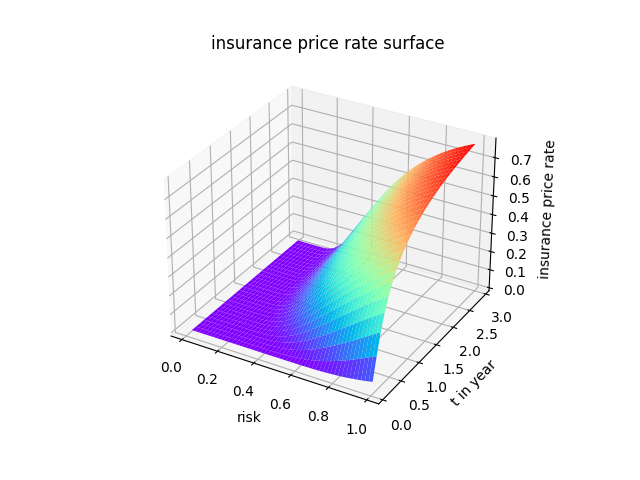
\includegraphics[width=\linewidth]{./graphs/insurance_price_rate_surface} % Figure image
	\caption{Price Changes with the Risk and Expiry Time} % Figure caption
	\label{fig:surface} % Label for referencing with \ref{bear}
\end{figure}

On the surface, the insurance price remains relatively low when the risk is less than 0.4, but it rapidly increases when the risk exceeds 0.4 and the expiry time reaches one year.
When the risk is close to 1.0, it signifies that people have lost faith in this DeFi protocol, and if you buy 100USDT coverage for three years, you will pay more than 70USDT.